\documentclass[a4paper]{article}
\usepackage[T1]{fontenc}
\usepackage[utf8]{inputenc}
\usepackage[french]{babel}
\usepackage{mathpazo}
\usepackage[scaled]{helvet}
\usepackage{courier}
\usepackage[margin=20mm]{geometry}
\usepackage{tabularx}
\usepackage{graphicx}
\usepackage{amsmath}


\makeatletter
\newenvironment{expl}{%
  \begin{list}{}{%
      \small\itshape%
      \topsep\z@%
      \listparindent0pt%\parindent%
      \parsep0.75\baselineskip%\parskip%
      \setlength{\leftmargin}{20mm}%
      \setlength{\rightmargin}{20mm}%
    }
  \item[]}%
  {\end{list}}
  


\makeatother

%\title{Rapport du Projet  \\ Intelligence Artificielle }
%\author{Abdelheq DELMI BOURAS \\ Siham JANATI }


%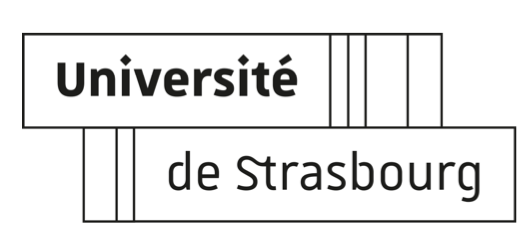
\includegraphics[width=\textwidth]{logo-unistra.png}\\





%\date{Mars 2021}

\begin{document}
\sloppy

\pagenumbering{arabic}


\begin{center}
\linespread{2}\huge\textbf{Projet Intelligence Artificielle\\} 
\large\textbf{Détection d’outliers par arbres de décisions}
\vspace{1.2in}
\end{center}

\begin{figure}[h]
    \centering
    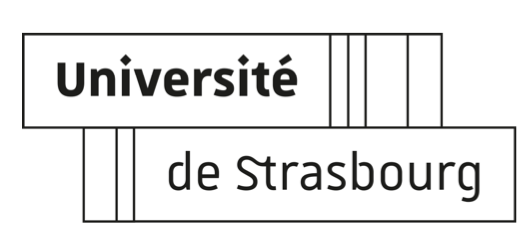
\includegraphics[width=0.8\textwidth]{logo-unistra.png}
\end{figure}

\begin{center}
\vspace{1.2in}\huge
\textbf{Siham JANATI \\
Abdelheq DELMI BOURAS }
\vspace{1.2in}

\large\textbf{L3-S6 Informatique \\ Université de Strasbourg}
\vspace{1.2in}

\textbf{Mars 2021}
\end{center}

\clearpage
\restoregeometry

%\maketitle


% Mettez une table des matières si votre rapport contient plus
% de 3 pages ou si vous ne suivez pas le plan suggéré :
%\tableofcontents

% supprimez toutes les explications comprises entre \begin{expl}
% et \end{expl} dans votre rapport.

\centering\section{Introduction}





Les outliers sont les données aberrantes présentes dans le jeu de données,\\c’est-à-dire les données dont la valeur s’éloigne significativement de la tendance\\ majoritaire obtenue à partir des autres données.\\
En data science, les outliers biaisent défavorablement les modèles s’ils ne \\sont pas pris en compte. Une manière (radicale !) de les gérer consiste à les supprimer\\ du jeu de données pour ne travailler qu’avec des valeurs régulières,aussi appelées inliers.\\
Dans ce projet, on se propose de détecter les outliers avec une méthode nonsupervisée.\\
Une vérité terrain est fournie mais cette dernière ne sera utilisée que pour l’évaluation.

\includegraphics[width=\textwidth]{figure0.png}\\


\newpage

\section{Préparation des données:}

\subsection{Recensement des données }\label{sec-shm}


\begin{center}
   \begin{tabular}{ | l | c | r | }
     \hline
     0 (inlier) & 250  \\ \hline
     1 (outlier) &80  \\ \hline
     %\hline
   \end{tabular}
 \end{center}

\subsection{Visualisation des données}
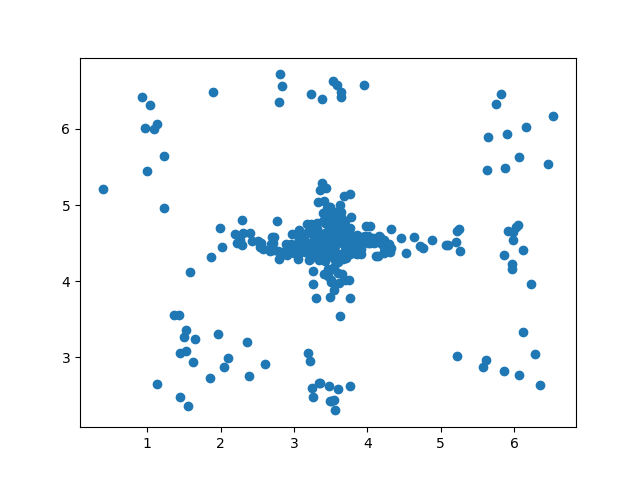
\includegraphics[width=\textwidth]{Figure_1.png}

\subsection{description des données:}

    dans la figure présentée ci-dessus, on aperçoit de manière approximative,  que les inliers se présentent dans la section  x[1,7:5,2]  et y[3,4:5,2]


\section{Évaluation}\label{evaluation}

\subsection{}

Le modèle semble bien détecter les inliers (
1000/1002 ), mais pas les outliers ( 5/35 ). Comme le but est de
détecter les outliers, le modèle ne semble pas si bon.\\

\subsection{}
\[ exactitude\
  = \dfrac{1000+2}{1000+2+30+5} = 0.97
\]
\[ exactitude \ pondéree
  = \dfrac{ \dfrac{5}{35} + \dfrac{1000}{1002}}{2} = 0.57
\]


\subsection{}
Parce que le modèle détecte bien les négatifs mais
pas les positifs. Et comme les données dont nous disposons comprennent
surtout des négatifs (inliers), l'exactitude semblera bonne.\\

\subsection{}

Elle n'est pas pertinente car elle ne renseigne pas
sur la capacité du modèle à détecter les outliers, ce qui est notre but.\\



\section{Algorithmes}\label{structures}

\subsection{Arbre Réduit à une feuille\\}




\begin{itemize}
\itemsep1pt\parskip0pt\parsep0pt
\item
  \textbf{DecisionLeaf}: une feuille de decision avec comme attributs

  \begin{itemize}
  \itemsep1pt\parskip0pt\parsep0pt
  \item
    \textbf{a} \texttt{higher\_split}
  \item
    \textbf{b} \texttt{lower\_split}
  \item
    \textbf{currentAttrib} \texttt{l'attribut d'intérêt}
  \item
    \textbf{D} \texttt{notre dataset\\}
  \end{itemize}
\end{itemize}


\includegraphics[width=\textwidth]{4_1}\\






\subsection{Arbre Artificiel}

\subsubsection{Structures}

Pour notre arbre superficiel, il nous faut créer 2 classes supplémentaires, qui sont
implémentées dans le fichier \texttt{'Node.py'}
\\


\begin{itemize}
\item
  \textbf{DecisionDirect}: Une classe de decision directe avec comme
  attributs

  \begin{itemize}
  \itemsep1pt\parskip0pt\parsep0pt
  \item
    \textbf{D} \texttt{notre dataset}
  \item
    \textbf{nb} \texttt{le nombre des exmples reste à traiters}
  \item
    \textbf{outier} \texttt{type Boolean\\}
  \end{itemize}
\end{itemize}

\includegraphics[width=\textwidth]{4_2}
\\
\begin{itemize}
\item
  \textbf{Node}: Une classe pour l'arbre artificiel, avec comme
  attributs
  \begin{itemize}
  \itemsep1pt\parskip0pt\parsep0pt
  \item
    \textbf{a} \texttt{higher\_split}
  \item
    \textbf{b} \texttt{lower\_split}
  \item
    \textbf{R} \texttt{sous-arbre/branche droit}
  \item
    \textbf{L} \texttt{sous-arbre/branche gauche}
  \item
    \textbf{C} \texttt{sous-arbre/branche du centre}
  \end{itemize}
\end{itemize}

\includegraphics[width=\textwidth]{4_3}


\subsubsection{Évaluation de l'arbre artificiel}


Feuille de Décision

\begin{figure}[htbp]
\centering
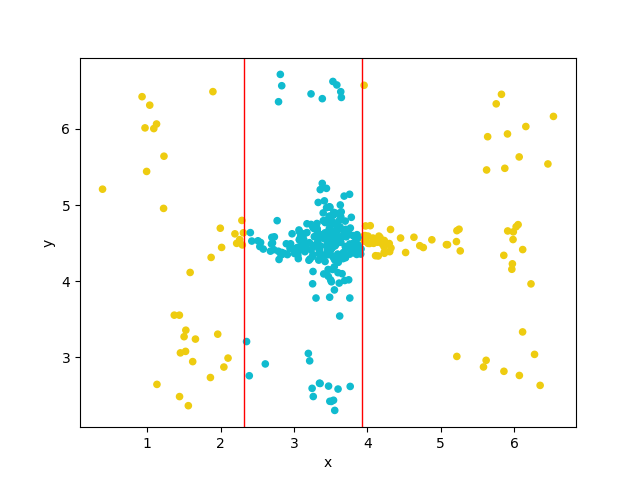
\includegraphics{eval1.png}
\caption{Decision Leaf}
\end{figure}

\begin{verbatim}
Exactitude: 0.7818181818181819
Exactitude pondérée: 0.74975
Précision: 0.5392156862745098
Rappel: 0.6875
\end{verbatim}

\newpage
\\
\begin{center}\rule{3in}{0.4pt}\end{center}

Arbre de décision:

\begin{figure}[]
\centering
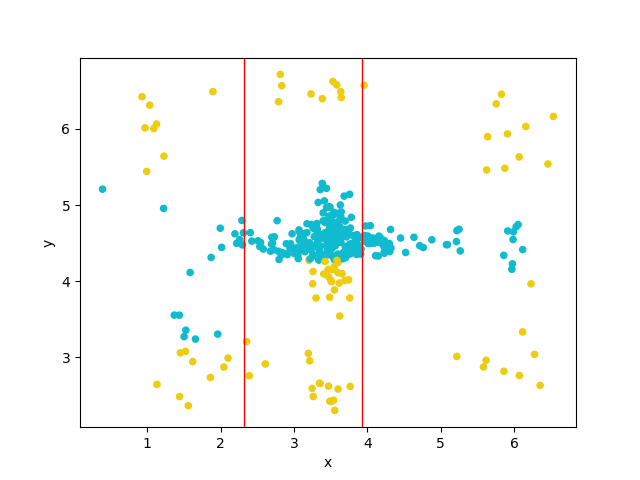
\includegraphics{eval2.png}
\caption{build Decision Tree}
\end{figure}

\begin{verbatim}
Exactitude: 0.8393939393939394
Exactitude pondérée: 0.8005
Précision: 0.651685393258427
Rappel: 0.725
\end{verbatim}

\begin{center}\rule{3in}{0.4pt}\end{center}

\paragraph{Commentaires:\\}\label{commentaires}

Les résultats se sont bien améliorés de la première évaluation avec un
\textbf{arbre réduit} à une feuille, avec un rappel de \texttt{0.76}, le
modèle \textbf{arbre artificiel} a réussi a bien détecter les
(in/out)liere à 80\%.\\

\newpage

\section{Arbre Généralisé}


\subsection{Adaptation de l'algorithme}

\subsection{Évaluation:}
\text{Feuille de décision:}\label{feuille-de-duxe9cision}

\begin{center}
   \begin{tabular}{ | l | c | r | }
     \hline
     exactitude pondérée & Précision  & Rappel \\ \hline
     0.74975 & 0.5392156862745098 &   0.6875  \\ \hline
     %\hline
   \end{tabular}
 \end{center}

\text{Arbre Superficiel:}\label{arbre-superficiel}

\begin{center}
   \begin{tabular}{ | l | c | r | }
     \hline
     exactitude pondérée & Précision  & Rappel \\ \hline
     0.8005 & 0.651685393258427 &    0.725  \\ \hline
     %\hline
   \end{tabular}
 \end{center}

\text{Arbre Généralisé:}\label{arbre-guxe9nuxe9ralisuxe9}

\begin{center}
   \begin{tabular}{ | l | c | r | d | }
     \hline
     Hauteur & exactitude pondérée & Précision  & Rappel \\ \hline
     1 & 0.74975 & 0.5392156862745098 &    0.6875  \\ \hline
     2 &0.804 & 0.5714285714285714 & 0.8 \\ \hline
     3 &0.5714999999999999 &0.2987012987012987 & 0.575 \\ \hline
     4 & 0.5175 & 0.2541436464088398 & 0.575 \\ \hline
     %\hline
   \end{tabular}
 \end{center}
 



\subsection{Meilleure hauteur!?}

Une hauteur de 2 donne les meilleurs résultats. Mais celle-ci n'est pas
meilleure en précision que les résultats de l'arbre superficiel de la
question 4-2, elle lui est égale en exactitude pondérée et est meilleure
en rappel. Donc elle est moins précise dans la détection des outliers
(plus de faux positifs), par contre elle détectera plus d'outliers que
l'arbre superficiel qui en manquera certains. Et ceci est tout à fait
normal, en améliorant le rappel on perdra un peu de précision.

\end{document}
